\documentclass[xcolor=svgnames,9pt,english,aspectratio=169,t]{beamer}
%\documentclass[xcolor=svgnames,9pt,english,handout,aspectratio=169,t]{beamer}
\newcommand{\handout}{0}

% =====================================================================
% POLI 450A (2026) --- shared TEMPLATE layer.
%
% Input from each lecture near the top of its file, BEFORE
% ../course_theme.tex (metropolis must be selected before the course
% palette overrides it):
%
%   \documentclass[xcolor=svgnames,9pt,english,aspectratio=169]{beamer}
%   \newcommand{\handout}{0}
%   % =====================================================================
% POLI 450A (2026) --- shared TEMPLATE layer.
%
% Input from each lecture near the top of its file, BEFORE
% ../course_theme.tex (metropolis must be selected before the course
% palette overrides it):
%
%   \documentclass[xcolor=svgnames,9pt,english,aspectratio=169]{beamer}
%   \newcommand{\handout}{0}
%   % =====================================================================
% POLI 450A (2026) --- shared TEMPLATE layer.
%
% Input from each lecture near the top of its file, BEFORE
% ../course_theme.tex (metropolis must be selected before the course
% palette overrides it):
%
%   \documentclass[xcolor=svgnames,9pt,english,aspectratio=169]{beamer}
%   \newcommand{\handout}{0}
%   \input{../course_preamble.tex}
%   \input{../course_theme.tex}
%   \graphicspath{{./}{./figs/}}
%   \title[Short title]{450A Political Methodology I}
%   \subtitle{Lecture N: ...}
%
% Modeled on the 2026 Northwestern workshop template
% (Teaching/PanelData/_latex/2026/202608_Northwestern/workshop_preamble.tex).
%
% SCOPE: theme, beamer layout, packages, the roadmap hooks, and --- unlike
% the Northwestern decks --- the notation macros. The 450A lectures
% grew from one common ancestor, so their macro blocks agree wherever they
% overlap; merging them is safe. Three points where they had drifted are
% resolved here, and each is flagged inline below.
% =====================================================================

\usetheme{metropolis}
\metroset{sectionpage=none, subsectionpage=none, numbering=none}
\setbeamertemplate{navigation symbols}{}

\setbeamersize{text margin left=5mm, text margin right=5mm}
\setbeamertemplate{itemize/enumerate body begin}{\leftmargini=1.5em\relax}
\setbeamertemplate{itemize/enumerate subbody begin}{\leftmarginii=1.5em\relax}
\setbeamertemplate{itemize/enumerate subsubbody begin}{\leftmarginiii=1.5em\relax}

% ----------------------------------------------------------- top alignment
% Every deck passes the t class option, so beamer applies the frame key
% below to every frame (explicit [plain,c] frames — title page, roadmaps —
% stay centered). Beamer's stock t key puts a rigid .2cm pad above the
% content; frames sized to this template's full-height ceilings then run
% Overfull \vbox by up to that pad. Same key as beamerbaseframe.sty, with
% one change: the pad may shrink to zero when the frame is full.
\makeatletter
\define@key{beamerframe}{t}[true]{% top
  \beamer@frametopskip=.2cm plus .5\paperheight minus .2cm\relax%
  \beamer@framebottomskip=0pt plus 1fill\relax%
  \beamer@frametopskipautobreak=\beamer@frametopskip\relax%
  \beamer@framebottomskipautobreak=\beamer@framebottomskip\relax%
}

% ------------------------------------------------- slide-top check (2026-10-11)
% A slide whose content is too tall for the frame is squeezed: the pad above
% shrinks and its content starts higher than on other slides, so a figure
% "wobbles" when the class steps from one slide to the next (Lecture 4-1,
% slides 1-2, 2026-10-11). The marker below records where each slide's
% content starts (a whatsit: it adds no space and moves nothing).
% `python3 ../check_slides.py lec<N>` then lists every slide that starts
% higher than the deck's normal position. That list must be empty.
% Recorded per slide: page, frame number, content-top y (sp), the room left
% below the title bar, and P for a plain frame (title page, roadmaps).
\providecommand\slidetop[5]{}
\AtBeginDocument{\immediate\write\@auxout{\string\providecommand\string\slidetop[5]{}}}
\def\beamer@markframetop{%
  \pdfsavepos
  \edef\beamer@marktmp{\noexpand\write\noexpand\@auxout{\string\slidetop
    {\noexpand\thepage}{\noexpand\insertframenumber}{\noexpand\the\noexpand\pdflastypos}%
    {\number\beamer@frametextheight}{\ifbeamer@plainframe P\else N\fi}}}%
  \beamer@marktmp}
\RequirePackage{etoolbox}
\patchcmd{\endbeamer@frameslide}
  {\vskip\beamer@frametopskip}
  {\vskip\beamer@frametopskip\beamer@markframetop}
  {}{\PackageWarning{course_preamble}{slide-top marker not installed}}
\makeatother

% ---------------------------------------------------------------- packages
\usepackage{xcolor}
\usepackage{colortbl}
\usepackage{amsmath}
\usepackage{amsfonts}
\usepackage{amssymb}
\usepackage{bm}
\usepackage{graphicx}
\usepackage{multirow}
\usepackage{fancyvrb}
\usepackage{listings}
\usepackage{tikz}
\usetikzlibrary{arrows.meta,positioning,decorations.pathreplacing}

% --------------------------------------------------------- figure fitting
% Default bounding box for every \includegraphics that does not override it.
% With keepaspectratio the image is scaled to fit *inside* width x height, so
% a figure can never run past the side margins or off the bottom of a slide.
% Options given at the call site override these on a per-key basis: e.g.
% [width=.6\linewidth] narrows the box but keeps the height ceiling.
% \figmaxheight is set at \begin{document}: beamer only computes the final
% \textheight once the head/foot templates are known. 0.80 is just under what a
% frame with a title and one line of text can hold (measured: 0.834\textheight);
% a frame that needs more room for text can lower it locally.
\newlength{\figmaxheight}
\AtBeginDocument{\setlength{\figmaxheight}{0.80\textheight}}
\setkeys{Gin}{width=\linewidth,height=\figmaxheight,keepaspectratio}

% -------------------------------------------------------- roadmap frames
% Identical in all lectures. A lecture that does not want the
% subsection roadmap clears it after the \input with \AtBeginSubsection[]{}.
% hideothersubsections is load-bearing, not cosmetic: lecture 4 had 13
% subsections before it was split into 4-1, 4-2 and 4-3 (2026-10-09), and a
% full contents list ran off the top and bottom of the slide. Hiding the other sections' subsections caps the list at 10 lines.
\subject{Talks}
% No back-to-back roadmaps (Yiqing, 2026-10-11): when a subsection starts right
% after its section's roadmap, with no content slide in between, its own
% roadmap would repeat the one just shown (5-1's handout showed "Two Cases"
% twice), so it is skipped. The section roadmap records the frame count; the
% subsection roadmap appears only if a content slide has come since.
\makeatletter
\def\course@secframe{-1}
\AtBeginSection[]
{
  \begin{frame}[plain,c]
    \frametitle{}
    \tableofcontents[currentsection,hideothersubsections]
    \addtocounter{framenumber}{-1}
  \end{frame}
  \xdef\course@secframe{\the\c@framenumber}
}
\AtBeginSubsection[]
{
  \ifnum\c@framenumber=\course@secframe\relax\else
  \begin{frame}[plain,c]
    \frametitle{}
    \tableofcontents[currentsection,currentsubsection,hideothersubsections]
    \addtocounter{framenumber}{-1}
  \end{frame}
  \fi
}
\makeatother

% ------------------------------------------------------ theorem environments
\newtheorem{assumption}{Assumption}
\newtheorem{iass}{Identification Assumption}
\newtheorem{ires}{Identification Result}
\newtheorem{estm}{Estimand}
\newtheorem{esti}{Estimator}
\newtheorem{question}{Question}
\newtheorem{answer}{Answer}
\newtheorem{proposition}{Proposition}

% =====================================================================
% Notation
% =====================================================================
\definecolor{dgreen}{rgb}{0,.6,0.8}

\renewcommand\r{\right}
\renewcommand\l{\left}
\newcommand{\bs}{\boldsymbol}
\newcommand{\mb}{\mathbf}
\newcommand{\real}{\mathbb{R}}
\newcommand{\cN}{\mathcal{N}}
\newcommand{\E}{\mathbb{E}}
\newcommand{\V}{\mathbb{V}}

% MERGE NOTE 1. Lecture 2-4 set \epsilon to \varepsilon; the other twelve
% left it at the upright default. Adopting \varepsilon course-wide so the
% error term looks the same in every lecture.
\renewcommand{\epsilon}{\varepsilon}

% MERGE NOTE 2. Lecture 2-4 wrote its vectors as \bm (bold italic); the other
% twelve use \mathbf (bold upright). \mathbf wins --- it is the convention in
% eleven of the thirteen decks and in the course's matrix lectures. Only
% \iid, \E, \cN and \Var from that block are actually used in 2-4's body.
\renewcommand{\u}{\ensuremath{\mb{u}}}
\renewcommand{\v}{\ensuremath{\mb{v}}}
\newcommand{\U}{\ensuremath{\mb{U}}}
\newcommand{\M}{\ensuremath{\mb{M}}}
\newcommand{\X}{\ensuremath{\mb{X}}}
\newcommand{\x}{\ensuremath{\mb{x}}}
\newcommand{\y}{\ensuremath{\mb{y}}}
\newcommand{\Z}{\ensuremath{\mb{Z}}}
\newcommand{\C}{\ensuremath{\mb{C}}}
\newcommand{\D}{\ensuremath{\mb{D}}}
\newcommand{\I}{\ensuremath{\mb{I}}}
\newcommand{\W}{\ensuremath{\mb{W}}}
\renewcommand{\a}{\ensuremath{\mb{a}}}
\renewcommand{\P}{\ensuremath{\mb{P}}}
\newcommand{\one}{\ensuremath{\mb{1}}}
\newcommand{\zero}{\ensuremath{\mb{0}}}

\renewcommand{\b}{\ensuremath{\bs{\beta}}}
\newcommand{\be}{\ensuremath{\bs{\beta}}}
\newcommand{\e}{\ensuremath{\bs{\epsilon}}}
\newcommand{\eps}{\ensuremath{\bs{\epsilon}}}
\newcommand{\eeta}{\ensuremath{\bs{\eta}}}
\newcommand{\bhat}{\ensuremath{\hat{\bs{\beta}}}}
\newcommand{\ehat}{\ensuremath{\hat{\e}}}
\newcommand{\Sig}{\ensuremath{\bs{\Sigma}}}
\newcommand{\SigInv}{\ensuremath{\bs{\Sigma^{-1}}}}

\newcommand{\XX}{\ensuremath{\X'\X}}
\newcommand{\XXinv}{\ensuremath{\left(\XX\right)^{-1}}}
\newcommand{\hatmat}{\ensuremath{\X \XXinv \X'}}
\newcommand{\hatsig}{\ensuremath{\hat{\sigma}^2}}
\newcommand{\sig}{\ensuremath{\sigma^2}}

\newcommand{\cA}{\mathcal{A}}
\newcommand{\cJ}{\mathcal{J}}
\newcommand{\cL}{\mathcal{L}}
\newcommand{\cLL}{\mathcal{LL}}
\newcommand{\cll}{\ell}
\newcommand{\cQ}{\mathcal{Q}}
\newcommand{\cP}{\mathcal{P}}

% MERGE NOTE 3. \var / \Var and \cov / \Cov were spelled with \text in some
% lectures and \mbox in others. Same output; \text kept.
\newcommand{\var}{\text{Var}}
\newcommand{\Var}{\text{Var}}
\newcommand{\cov}{\text{Cov}}
\newcommand{\Cov}{\text{Cov}}
\newcommand{\cor}{\text{Cor}}
\newcommand{\tr}{\text{tr}}
\newcommand{\avepop}{\frac{1}{n}\sum_{i=1}^n}

\DeclareMathOperator*\plim{plim}
\DeclareMathOperator\rank{rank}
\DeclareMathOperator*\argmax{argmax}
\DeclareMathOperator*\argmin{argmin}
\DeclareMathOperator{\sgn}{sgn}
\newcommand{\diag}{\mathop{\mathrm{diag}}}

\newcommand\ud{\mathrm{d}}
\newcommand\dist{\buildrel\rm d\over\sim}
\newcommand\ind{\stackrel{\rm indep.}{\sim}}
\newcommand\iid{\stackrel{\rm i.i.d.}{\sim}}
\newcommand\logit{{\rm logit}}

\newcommand\indep{\protect\mathpalette{\protect\independenT}{\perp}}
\def\independenT#1#2{\mathrel{\rlap{$#1#2$}\mkern2mu{#1#2}}}

% ------------------------------------------------------------- text helpers
\newcommand{\bi}{\begin{itemize}}
\newcommand{\ei}{\end{itemize}}
\newcommand{\noi}{\noindent}
\newcommand{\red}{\textcolor{Cardinal}}
\newcommand{\blue}{\textcolor{CourseBlue}}
\newcommand{\gray}{\textcolor{gray}}
\newcommand\spacingset[1]{\renewcommand{\baselinestretch}{#1}\small\normalsize}

\hyphenation{tyamamot}


% ------------------------------------------------ figure-position check (2026-10-11)
% Records where every \includegraphics lands and its size (a whatsit; it moves
% nothing). check_slides.py flags two consecutive slides that show a figure of
% the same size in different places: the class sees it jump (Lecture 3, slides
% 18 to 19: one frame had \vspace{.3cm} above the figure, the next did not),
% and two consecutive slides that show the same file at different sizes or
% places (Lecture 6-3, slides 10 to 11, the ballot image). The file name is the
% seventh field.
\makeatletter
\providecommand\figpos[7]{}
\AtBeginDocument{\immediate\write\@auxout{\string\providecommand\string\figpos[7]{}}}
\newbox\course@figbox
\let\course@origGinclude\Ginclude@graphics
\def\Ginclude@graphics#1{%
  \setbox\course@figbox\hbox{\course@origGinclude{#1}}%
  \pdfsavepos
  \edef\course@figtmp{\noexpand\write\noexpand\@auxout{\string\figpos
    {\noexpand\thepage}{\noexpand\insertframenumber}%
    {\noexpand\the\noexpand\pdflastxpos}{\noexpand\the\noexpand\pdflastypos}%
    {\number\wd\course@figbox}{\number\ht\course@figbox}{\detokenize{#1}}}}%
  \course@figtmp
  \box\course@figbox}
\makeatother

%   % =====================================================================
% POLI 450A (2026) --- shared visual system.
% Input from each lecture AFTER ../course_preamble.tex.
%
% Same shape as the 2026 Northwestern workshop theme
% (Teaching/PanelData/_latex/2026/202608_Northwestern/workshop_theme.tex),
% with the workshop's purple swapped for the course's cardinal. Kept
% deliberately light so the lecture sources stay easy to edit.
%
% To retune the course to Stanford's official cardinal, change the one
% Cardinal line below to HTML 8C1515.
% =====================================================================
\definecolor{Cardinal}{HTML}{A8003B}     % primary: titles, structure, alerts
\definecolor{CourseInk}{HTML}{252A34}    % body text
\definecolor{CourseBlue}{HTML}{2F6B9A}   % secondary accent
\definecolor{CourseMist}{HTML}{F8F1F4}   % block backgrounds

\setbeamercolor{normal text}{fg=CourseInk,bg=white}
\setbeamercolor{structure}{fg=Cardinal}
\setbeamercolor{alerted text}{fg=Cardinal}
\setbeamercolor{frametitle}{fg=white,bg=Cardinal}
\setbeamercolor{title}{fg=Cardinal}
\setbeamercolor{subtitle}{fg=CourseInk}
\setbeamercolor{block title}{fg=white,bg=Cardinal}
\setbeamercolor{block body}{fg=CourseInk,bg=CourseMist}
\setbeamercolor{section in toc}{fg=Cardinal}
\setbeamercolor{subsection in toc}{fg=CourseInk}
\setbeamercolor{itemize item}{fg=Cardinal}
\setbeamercolor{itemize subitem}{fg=Cardinal}
\setbeamercolor{enumerate item}{fg=Cardinal}

\setbeamerfont{title}{series=\bfseries,size=\Large}
\setbeamerfont{frametitle}{series=\bfseries,size=\large}
\setbeamerfont{block title}{series=\bfseries}
\setbeamertemplate{navigation symbols}{}
\setbeamertemplate{items}[circle]
\setbeamertemplate{blocks}[rounded][shadow=false]
\setbeamertemplate{frametitle continuation}{}
\setbeamertemplate{footline}{%
  \leavevmode\hbox{%
  \begin{beamercolorbox}[wd=.88\paperwidth,ht=2.6ex,dp=1.2ex,leftskip=1.2em]{author in head/foot}%
  \usebeamerfont{author in head/foot}\insertshorttitle
  \end{beamercolorbox}%
  \begin{beamercolorbox}[wd=.12\paperwidth,ht=2.6ex,dp=1.2ex,center]{date in head/foot}%
  \insertframenumber
  \end{beamercolorbox}}}

\newcommand{\slidesource}[1]{\vfill{\scriptsize\color{gray}Source: #1}}
\newcommand{\keyquestion}[1]{\begin{block}{Question}#1\end{block}}

%   \graphicspath{{./}{./figs/}}
%   \title[Short title]{450A Political Methodology I}
%   \subtitle{Lecture N: ...}
%
% Modeled on the 2026 Northwestern workshop template
% (Teaching/PanelData/_latex/2026/202608_Northwestern/workshop_preamble.tex).
%
% SCOPE: theme, beamer layout, packages, the roadmap hooks, and --- unlike
% the Northwestern decks --- the notation macros. The 450A lectures
% grew from one common ancestor, so their macro blocks agree wherever they
% overlap; merging them is safe. Three points where they had drifted are
% resolved here, and each is flagged inline below.
% =====================================================================

\usetheme{metropolis}
\metroset{sectionpage=none, subsectionpage=none, numbering=none}
\setbeamertemplate{navigation symbols}{}

\setbeamersize{text margin left=5mm, text margin right=5mm}
\setbeamertemplate{itemize/enumerate body begin}{\leftmargini=1.5em\relax}
\setbeamertemplate{itemize/enumerate subbody begin}{\leftmarginii=1.5em\relax}
\setbeamertemplate{itemize/enumerate subsubbody begin}{\leftmarginiii=1.5em\relax}

% ----------------------------------------------------------- top alignment
% Every deck passes the t class option, so beamer applies the frame key
% below to every frame (explicit [plain,c] frames — title page, roadmaps —
% stay centered). Beamer's stock t key puts a rigid .2cm pad above the
% content; frames sized to this template's full-height ceilings then run
% Overfull \vbox by up to that pad. Same key as beamerbaseframe.sty, with
% one change: the pad may shrink to zero when the frame is full.
\makeatletter
\define@key{beamerframe}{t}[true]{% top
  \beamer@frametopskip=.2cm plus .5\paperheight minus .2cm\relax%
  \beamer@framebottomskip=0pt plus 1fill\relax%
  \beamer@frametopskipautobreak=\beamer@frametopskip\relax%
  \beamer@framebottomskipautobreak=\beamer@framebottomskip\relax%
}

% ------------------------------------------------- slide-top check (2026-10-11)
% A slide whose content is too tall for the frame is squeezed: the pad above
% shrinks and its content starts higher than on other slides, so a figure
% "wobbles" when the class steps from one slide to the next (Lecture 4-1,
% slides 1-2, 2026-10-11). The marker below records where each slide's
% content starts (a whatsit: it adds no space and moves nothing).
% `python3 ../check_slides.py lec<N>` then lists every slide that starts
% higher than the deck's normal position. That list must be empty.
% Recorded per slide: page, frame number, content-top y (sp), the room left
% below the title bar, and P for a plain frame (title page, roadmaps).
\providecommand\slidetop[5]{}
\AtBeginDocument{\immediate\write\@auxout{\string\providecommand\string\slidetop[5]{}}}
\def\beamer@markframetop{%
  \pdfsavepos
  \edef\beamer@marktmp{\noexpand\write\noexpand\@auxout{\string\slidetop
    {\noexpand\thepage}{\noexpand\insertframenumber}{\noexpand\the\noexpand\pdflastypos}%
    {\number\beamer@frametextheight}{\ifbeamer@plainframe P\else N\fi}}}%
  \beamer@marktmp}
\RequirePackage{etoolbox}
\patchcmd{\endbeamer@frameslide}
  {\vskip\beamer@frametopskip}
  {\vskip\beamer@frametopskip\beamer@markframetop}
  {}{\PackageWarning{course_preamble}{slide-top marker not installed}}
\makeatother

% ---------------------------------------------------------------- packages
\usepackage{xcolor}
\usepackage{colortbl}
\usepackage{amsmath}
\usepackage{amsfonts}
\usepackage{amssymb}
\usepackage{bm}
\usepackage{graphicx}
\usepackage{multirow}
\usepackage{fancyvrb}
\usepackage{listings}
\usepackage{tikz}
\usetikzlibrary{arrows.meta,positioning,decorations.pathreplacing}

% --------------------------------------------------------- figure fitting
% Default bounding box for every \includegraphics that does not override it.
% With keepaspectratio the image is scaled to fit *inside* width x height, so
% a figure can never run past the side margins or off the bottom of a slide.
% Options given at the call site override these on a per-key basis: e.g.
% [width=.6\linewidth] narrows the box but keeps the height ceiling.
% \figmaxheight is set at \begin{document}: beamer only computes the final
% \textheight once the head/foot templates are known. 0.80 is just under what a
% frame with a title and one line of text can hold (measured: 0.834\textheight);
% a frame that needs more room for text can lower it locally.
\newlength{\figmaxheight}
\AtBeginDocument{\setlength{\figmaxheight}{0.80\textheight}}
\setkeys{Gin}{width=\linewidth,height=\figmaxheight,keepaspectratio}

% -------------------------------------------------------- roadmap frames
% Identical in all lectures. A lecture that does not want the
% subsection roadmap clears it after the \input with \AtBeginSubsection[]{}.
% hideothersubsections is load-bearing, not cosmetic: lecture 4 had 13
% subsections before it was split into 4-1, 4-2 and 4-3 (2026-10-09), and a
% full contents list ran off the top and bottom of the slide. Hiding the other sections' subsections caps the list at 10 lines.
\subject{Talks}
% No back-to-back roadmaps (Yiqing, 2026-10-11): when a subsection starts right
% after its section's roadmap, with no content slide in between, its own
% roadmap would repeat the one just shown (5-1's handout showed "Two Cases"
% twice), so it is skipped. The section roadmap records the frame count; the
% subsection roadmap appears only if a content slide has come since.
\makeatletter
\def\course@secframe{-1}
\AtBeginSection[]
{
  \begin{frame}[plain,c]
    \frametitle{}
    \tableofcontents[currentsection,hideothersubsections]
    \addtocounter{framenumber}{-1}
  \end{frame}
  \xdef\course@secframe{\the\c@framenumber}
}
\AtBeginSubsection[]
{
  \ifnum\c@framenumber=\course@secframe\relax\else
  \begin{frame}[plain,c]
    \frametitle{}
    \tableofcontents[currentsection,currentsubsection,hideothersubsections]
    \addtocounter{framenumber}{-1}
  \end{frame}
  \fi
}
\makeatother

% ------------------------------------------------------ theorem environments
\newtheorem{assumption}{Assumption}
\newtheorem{iass}{Identification Assumption}
\newtheorem{ires}{Identification Result}
\newtheorem{estm}{Estimand}
\newtheorem{esti}{Estimator}
\newtheorem{question}{Question}
\newtheorem{answer}{Answer}
\newtheorem{proposition}{Proposition}

% =====================================================================
% Notation
% =====================================================================
\definecolor{dgreen}{rgb}{0,.6,0.8}

\renewcommand\r{\right}
\renewcommand\l{\left}
\newcommand{\bs}{\boldsymbol}
\newcommand{\mb}{\mathbf}
\newcommand{\real}{\mathbb{R}}
\newcommand{\cN}{\mathcal{N}}
\newcommand{\E}{\mathbb{E}}
\newcommand{\V}{\mathbb{V}}

% MERGE NOTE 1. Lecture 2-4 set \epsilon to \varepsilon; the other twelve
% left it at the upright default. Adopting \varepsilon course-wide so the
% error term looks the same in every lecture.
\renewcommand{\epsilon}{\varepsilon}

% MERGE NOTE 2. Lecture 2-4 wrote its vectors as \bm (bold italic); the other
% twelve use \mathbf (bold upright). \mathbf wins --- it is the convention in
% eleven of the thirteen decks and in the course's matrix lectures. Only
% \iid, \E, \cN and \Var from that block are actually used in 2-4's body.
\renewcommand{\u}{\ensuremath{\mb{u}}}
\renewcommand{\v}{\ensuremath{\mb{v}}}
\newcommand{\U}{\ensuremath{\mb{U}}}
\newcommand{\M}{\ensuremath{\mb{M}}}
\newcommand{\X}{\ensuremath{\mb{X}}}
\newcommand{\x}{\ensuremath{\mb{x}}}
\newcommand{\y}{\ensuremath{\mb{y}}}
\newcommand{\Z}{\ensuremath{\mb{Z}}}
\newcommand{\C}{\ensuremath{\mb{C}}}
\newcommand{\D}{\ensuremath{\mb{D}}}
\newcommand{\I}{\ensuremath{\mb{I}}}
\newcommand{\W}{\ensuremath{\mb{W}}}
\renewcommand{\a}{\ensuremath{\mb{a}}}
\renewcommand{\P}{\ensuremath{\mb{P}}}
\newcommand{\one}{\ensuremath{\mb{1}}}
\newcommand{\zero}{\ensuremath{\mb{0}}}

\renewcommand{\b}{\ensuremath{\bs{\beta}}}
\newcommand{\be}{\ensuremath{\bs{\beta}}}
\newcommand{\e}{\ensuremath{\bs{\epsilon}}}
\newcommand{\eps}{\ensuremath{\bs{\epsilon}}}
\newcommand{\eeta}{\ensuremath{\bs{\eta}}}
\newcommand{\bhat}{\ensuremath{\hat{\bs{\beta}}}}
\newcommand{\ehat}{\ensuremath{\hat{\e}}}
\newcommand{\Sig}{\ensuremath{\bs{\Sigma}}}
\newcommand{\SigInv}{\ensuremath{\bs{\Sigma^{-1}}}}

\newcommand{\XX}{\ensuremath{\X'\X}}
\newcommand{\XXinv}{\ensuremath{\left(\XX\right)^{-1}}}
\newcommand{\hatmat}{\ensuremath{\X \XXinv \X'}}
\newcommand{\hatsig}{\ensuremath{\hat{\sigma}^2}}
\newcommand{\sig}{\ensuremath{\sigma^2}}

\newcommand{\cA}{\mathcal{A}}
\newcommand{\cJ}{\mathcal{J}}
\newcommand{\cL}{\mathcal{L}}
\newcommand{\cLL}{\mathcal{LL}}
\newcommand{\cll}{\ell}
\newcommand{\cQ}{\mathcal{Q}}
\newcommand{\cP}{\mathcal{P}}

% MERGE NOTE 3. \var / \Var and \cov / \Cov were spelled with \text in some
% lectures and \mbox in others. Same output; \text kept.
\newcommand{\var}{\text{Var}}
\newcommand{\Var}{\text{Var}}
\newcommand{\cov}{\text{Cov}}
\newcommand{\Cov}{\text{Cov}}
\newcommand{\cor}{\text{Cor}}
\newcommand{\tr}{\text{tr}}
\newcommand{\avepop}{\frac{1}{n}\sum_{i=1}^n}

\DeclareMathOperator*\plim{plim}
\DeclareMathOperator\rank{rank}
\DeclareMathOperator*\argmax{argmax}
\DeclareMathOperator*\argmin{argmin}
\DeclareMathOperator{\sgn}{sgn}
\newcommand{\diag}{\mathop{\mathrm{diag}}}

\newcommand\ud{\mathrm{d}}
\newcommand\dist{\buildrel\rm d\over\sim}
\newcommand\ind{\stackrel{\rm indep.}{\sim}}
\newcommand\iid{\stackrel{\rm i.i.d.}{\sim}}
\newcommand\logit{{\rm logit}}

\newcommand\indep{\protect\mathpalette{\protect\independenT}{\perp}}
\def\independenT#1#2{\mathrel{\rlap{$#1#2$}\mkern2mu{#1#2}}}

% ------------------------------------------------------------- text helpers
\newcommand{\bi}{\begin{itemize}}
\newcommand{\ei}{\end{itemize}}
\newcommand{\noi}{\noindent}
\newcommand{\red}{\textcolor{Cardinal}}
\newcommand{\blue}{\textcolor{CourseBlue}}
\newcommand{\gray}{\textcolor{gray}}
\newcommand\spacingset[1]{\renewcommand{\baselinestretch}{#1}\small\normalsize}

\hyphenation{tyamamot}


% ------------------------------------------------ figure-position check (2026-10-11)
% Records where every \includegraphics lands and its size (a whatsit; it moves
% nothing). check_slides.py flags two consecutive slides that show a figure of
% the same size in different places: the class sees it jump (Lecture 3, slides
% 18 to 19: one frame had \vspace{.3cm} above the figure, the next did not),
% and two consecutive slides that show the same file at different sizes or
% places (Lecture 6-3, slides 10 to 11, the ballot image). The file name is the
% seventh field.
\makeatletter
\providecommand\figpos[7]{}
\AtBeginDocument{\immediate\write\@auxout{\string\providecommand\string\figpos[7]{}}}
\newbox\course@figbox
\let\course@origGinclude\Ginclude@graphics
\def\Ginclude@graphics#1{%
  \setbox\course@figbox\hbox{\course@origGinclude{#1}}%
  \pdfsavepos
  \edef\course@figtmp{\noexpand\write\noexpand\@auxout{\string\figpos
    {\noexpand\thepage}{\noexpand\insertframenumber}%
    {\noexpand\the\noexpand\pdflastxpos}{\noexpand\the\noexpand\pdflastypos}%
    {\number\wd\course@figbox}{\number\ht\course@figbox}{\detokenize{#1}}}}%
  \course@figtmp
  \box\course@figbox}
\makeatother

%   % =====================================================================
% POLI 450A (2026) --- shared visual system.
% Input from each lecture AFTER ../course_preamble.tex.
%
% Same shape as the 2026 Northwestern workshop theme
% (Teaching/PanelData/_latex/2026/202608_Northwestern/workshop_theme.tex),
% with the workshop's purple swapped for the course's cardinal. Kept
% deliberately light so the lecture sources stay easy to edit.
%
% To retune the course to Stanford's official cardinal, change the one
% Cardinal line below to HTML 8C1515.
% =====================================================================
\definecolor{Cardinal}{HTML}{A8003B}     % primary: titles, structure, alerts
\definecolor{CourseInk}{HTML}{252A34}    % body text
\definecolor{CourseBlue}{HTML}{2F6B9A}   % secondary accent
\definecolor{CourseMist}{HTML}{F8F1F4}   % block backgrounds

\setbeamercolor{normal text}{fg=CourseInk,bg=white}
\setbeamercolor{structure}{fg=Cardinal}
\setbeamercolor{alerted text}{fg=Cardinal}
\setbeamercolor{frametitle}{fg=white,bg=Cardinal}
\setbeamercolor{title}{fg=Cardinal}
\setbeamercolor{subtitle}{fg=CourseInk}
\setbeamercolor{block title}{fg=white,bg=Cardinal}
\setbeamercolor{block body}{fg=CourseInk,bg=CourseMist}
\setbeamercolor{section in toc}{fg=Cardinal}
\setbeamercolor{subsection in toc}{fg=CourseInk}
\setbeamercolor{itemize item}{fg=Cardinal}
\setbeamercolor{itemize subitem}{fg=Cardinal}
\setbeamercolor{enumerate item}{fg=Cardinal}

\setbeamerfont{title}{series=\bfseries,size=\Large}
\setbeamerfont{frametitle}{series=\bfseries,size=\large}
\setbeamerfont{block title}{series=\bfseries}
\setbeamertemplate{navigation symbols}{}
\setbeamertemplate{items}[circle]
\setbeamertemplate{blocks}[rounded][shadow=false]
\setbeamertemplate{frametitle continuation}{}
\setbeamertemplate{footline}{%
  \leavevmode\hbox{%
  \begin{beamercolorbox}[wd=.88\paperwidth,ht=2.6ex,dp=1.2ex,leftskip=1.2em]{author in head/foot}%
  \usebeamerfont{author in head/foot}\insertshorttitle
  \end{beamercolorbox}%
  \begin{beamercolorbox}[wd=.12\paperwidth,ht=2.6ex,dp=1.2ex,center]{date in head/foot}%
  \insertframenumber
  \end{beamercolorbox}}}

\newcommand{\slidesource}[1]{\vfill{\scriptsize\color{gray}Source: #1}}
\newcommand{\keyquestion}[1]{\begin{block}{Question}#1\end{block}}

%   \graphicspath{{./}{./figs/}}
%   \title[Short title]{450A Political Methodology I}
%   \subtitle{Lecture N: ...}
%
% Modeled on the 2026 Northwestern workshop template
% (Teaching/PanelData/_latex/2026/202608_Northwestern/workshop_preamble.tex).
%
% SCOPE: theme, beamer layout, packages, the roadmap hooks, and --- unlike
% the Northwestern decks --- the notation macros. The 450A lectures
% grew from one common ancestor, so their macro blocks agree wherever they
% overlap; merging them is safe. Three points where they had drifted are
% resolved here, and each is flagged inline below.
% =====================================================================

\usetheme{metropolis}
\metroset{sectionpage=none, subsectionpage=none, numbering=none}
\setbeamertemplate{navigation symbols}{}

\setbeamersize{text margin left=5mm, text margin right=5mm}
\setbeamertemplate{itemize/enumerate body begin}{\leftmargini=1.5em\relax}
\setbeamertemplate{itemize/enumerate subbody begin}{\leftmarginii=1.5em\relax}
\setbeamertemplate{itemize/enumerate subsubbody begin}{\leftmarginiii=1.5em\relax}

% ----------------------------------------------------------- top alignment
% Every deck passes the t class option, so beamer applies the frame key
% below to every frame (explicit [plain,c] frames — title page, roadmaps —
% stay centered). Beamer's stock t key puts a rigid .2cm pad above the
% content; frames sized to this template's full-height ceilings then run
% Overfull \vbox by up to that pad. Same key as beamerbaseframe.sty, with
% one change: the pad may shrink to zero when the frame is full.
\makeatletter
\define@key{beamerframe}{t}[true]{% top
  \beamer@frametopskip=.2cm plus .5\paperheight minus .2cm\relax%
  \beamer@framebottomskip=0pt plus 1fill\relax%
  \beamer@frametopskipautobreak=\beamer@frametopskip\relax%
  \beamer@framebottomskipautobreak=\beamer@framebottomskip\relax%
}

% ------------------------------------------------- slide-top check (2026-10-11)
% A slide whose content is too tall for the frame is squeezed: the pad above
% shrinks and its content starts higher than on other slides, so a figure
% "wobbles" when the class steps from one slide to the next (Lecture 4-1,
% slides 1-2, 2026-10-11). The marker below records where each slide's
% content starts (a whatsit: it adds no space and moves nothing).
% `python3 ../check_slides.py lec<N>` then lists every slide that starts
% higher than the deck's normal position. That list must be empty.
% Recorded per slide: page, frame number, content-top y (sp), the room left
% below the title bar, and P for a plain frame (title page, roadmaps).
\providecommand\slidetop[5]{}
\AtBeginDocument{\immediate\write\@auxout{\string\providecommand\string\slidetop[5]{}}}
\def\beamer@markframetop{%
  \pdfsavepos
  \edef\beamer@marktmp{\noexpand\write\noexpand\@auxout{\string\slidetop
    {\noexpand\thepage}{\noexpand\insertframenumber}{\noexpand\the\noexpand\pdflastypos}%
    {\number\beamer@frametextheight}{\ifbeamer@plainframe P\else N\fi}}}%
  \beamer@marktmp}
\RequirePackage{etoolbox}
\patchcmd{\endbeamer@frameslide}
  {\vskip\beamer@frametopskip}
  {\vskip\beamer@frametopskip\beamer@markframetop}
  {}{\PackageWarning{course_preamble}{slide-top marker not installed}}
\makeatother

% ---------------------------------------------------------------- packages
\usepackage{xcolor}
\usepackage{colortbl}
\usepackage{amsmath}
\usepackage{amsfonts}
\usepackage{amssymb}
\usepackage{bm}
\usepackage{graphicx}
\usepackage{multirow}
\usepackage{fancyvrb}
\usepackage{listings}
\usepackage{tikz}
\usetikzlibrary{arrows.meta,positioning,decorations.pathreplacing}

% --------------------------------------------------------- figure fitting
% Default bounding box for every \includegraphics that does not override it.
% With keepaspectratio the image is scaled to fit *inside* width x height, so
% a figure can never run past the side margins or off the bottom of a slide.
% Options given at the call site override these on a per-key basis: e.g.
% [width=.6\linewidth] narrows the box but keeps the height ceiling.
% \figmaxheight is set at \begin{document}: beamer only computes the final
% \textheight once the head/foot templates are known. 0.80 is just under what a
% frame with a title and one line of text can hold (measured: 0.834\textheight);
% a frame that needs more room for text can lower it locally.
\newlength{\figmaxheight}
\AtBeginDocument{\setlength{\figmaxheight}{0.80\textheight}}
\setkeys{Gin}{width=\linewidth,height=\figmaxheight,keepaspectratio}

% -------------------------------------------------------- roadmap frames
% Identical in all lectures. A lecture that does not want the
% subsection roadmap clears it after the \input with \AtBeginSubsection[]{}.
% hideothersubsections is load-bearing, not cosmetic: lecture 4 had 13
% subsections before it was split into 4-1, 4-2 and 4-3 (2026-10-09), and a
% full contents list ran off the top and bottom of the slide. Hiding the other sections' subsections caps the list at 10 lines.
\subject{Talks}
% No back-to-back roadmaps (Yiqing, 2026-10-11): when a subsection starts right
% after its section's roadmap, with no content slide in between, its own
% roadmap would repeat the one just shown (5-1's handout showed "Two Cases"
% twice), so it is skipped. The section roadmap records the frame count; the
% subsection roadmap appears only if a content slide has come since.
\makeatletter
\def\course@secframe{-1}
\AtBeginSection[]
{
  \begin{frame}[plain,c]
    \frametitle{}
    \tableofcontents[currentsection,hideothersubsections]
    \addtocounter{framenumber}{-1}
  \end{frame}
  \xdef\course@secframe{\the\c@framenumber}
}
\AtBeginSubsection[]
{
  \ifnum\c@framenumber=\course@secframe\relax\else
  \begin{frame}[plain,c]
    \frametitle{}
    \tableofcontents[currentsection,currentsubsection,hideothersubsections]
    \addtocounter{framenumber}{-1}
  \end{frame}
  \fi
}
\makeatother

% ------------------------------------------------------ theorem environments
\newtheorem{assumption}{Assumption}
\newtheorem{iass}{Identification Assumption}
\newtheorem{ires}{Identification Result}
\newtheorem{estm}{Estimand}
\newtheorem{esti}{Estimator}
\newtheorem{question}{Question}
\newtheorem{answer}{Answer}
\newtheorem{proposition}{Proposition}

% =====================================================================
% Notation
% =====================================================================
\definecolor{dgreen}{rgb}{0,.6,0.8}

\renewcommand\r{\right}
\renewcommand\l{\left}
\newcommand{\bs}{\boldsymbol}
\newcommand{\mb}{\mathbf}
\newcommand{\real}{\mathbb{R}}
\newcommand{\cN}{\mathcal{N}}
\newcommand{\E}{\mathbb{E}}
\newcommand{\V}{\mathbb{V}}

% MERGE NOTE 1. Lecture 2-4 set \epsilon to \varepsilon; the other twelve
% left it at the upright default. Adopting \varepsilon course-wide so the
% error term looks the same in every lecture.
\renewcommand{\epsilon}{\varepsilon}

% MERGE NOTE 2. Lecture 2-4 wrote its vectors as \bm (bold italic); the other
% twelve use \mathbf (bold upright). \mathbf wins --- it is the convention in
% eleven of the thirteen decks and in the course's matrix lectures. Only
% \iid, \E, \cN and \Var from that block are actually used in 2-4's body.
\renewcommand{\u}{\ensuremath{\mb{u}}}
\renewcommand{\v}{\ensuremath{\mb{v}}}
\newcommand{\U}{\ensuremath{\mb{U}}}
\newcommand{\M}{\ensuremath{\mb{M}}}
\newcommand{\X}{\ensuremath{\mb{X}}}
\newcommand{\x}{\ensuremath{\mb{x}}}
\newcommand{\y}{\ensuremath{\mb{y}}}
\newcommand{\Z}{\ensuremath{\mb{Z}}}
\newcommand{\C}{\ensuremath{\mb{C}}}
\newcommand{\D}{\ensuremath{\mb{D}}}
\newcommand{\I}{\ensuremath{\mb{I}}}
\newcommand{\W}{\ensuremath{\mb{W}}}
\renewcommand{\a}{\ensuremath{\mb{a}}}
\renewcommand{\P}{\ensuremath{\mb{P}}}
\newcommand{\one}{\ensuremath{\mb{1}}}
\newcommand{\zero}{\ensuremath{\mb{0}}}

\renewcommand{\b}{\ensuremath{\bs{\beta}}}
\newcommand{\be}{\ensuremath{\bs{\beta}}}
\newcommand{\e}{\ensuremath{\bs{\epsilon}}}
\newcommand{\eps}{\ensuremath{\bs{\epsilon}}}
\newcommand{\eeta}{\ensuremath{\bs{\eta}}}
\newcommand{\bhat}{\ensuremath{\hat{\bs{\beta}}}}
\newcommand{\ehat}{\ensuremath{\hat{\e}}}
\newcommand{\Sig}{\ensuremath{\bs{\Sigma}}}
\newcommand{\SigInv}{\ensuremath{\bs{\Sigma^{-1}}}}

\newcommand{\XX}{\ensuremath{\X'\X}}
\newcommand{\XXinv}{\ensuremath{\left(\XX\right)^{-1}}}
\newcommand{\hatmat}{\ensuremath{\X \XXinv \X'}}
\newcommand{\hatsig}{\ensuremath{\hat{\sigma}^2}}
\newcommand{\sig}{\ensuremath{\sigma^2}}

\newcommand{\cA}{\mathcal{A}}
\newcommand{\cJ}{\mathcal{J}}
\newcommand{\cL}{\mathcal{L}}
\newcommand{\cLL}{\mathcal{LL}}
\newcommand{\cll}{\ell}
\newcommand{\cQ}{\mathcal{Q}}
\newcommand{\cP}{\mathcal{P}}

% MERGE NOTE 3. \var / \Var and \cov / \Cov were spelled with \text in some
% lectures and \mbox in others. Same output; \text kept.
\newcommand{\var}{\text{Var}}
\newcommand{\Var}{\text{Var}}
\newcommand{\cov}{\text{Cov}}
\newcommand{\Cov}{\text{Cov}}
\newcommand{\cor}{\text{Cor}}
\newcommand{\tr}{\text{tr}}
\newcommand{\avepop}{\frac{1}{n}\sum_{i=1}^n}

\DeclareMathOperator*\plim{plim}
\DeclareMathOperator\rank{rank}
\DeclareMathOperator*\argmax{argmax}
\DeclareMathOperator*\argmin{argmin}
\DeclareMathOperator{\sgn}{sgn}
\newcommand{\diag}{\mathop{\mathrm{diag}}}

\newcommand\ud{\mathrm{d}}
\newcommand\dist{\buildrel\rm d\over\sim}
\newcommand\ind{\stackrel{\rm indep.}{\sim}}
\newcommand\iid{\stackrel{\rm i.i.d.}{\sim}}
\newcommand\logit{{\rm logit}}

\newcommand\indep{\protect\mathpalette{\protect\independenT}{\perp}}
\def\independenT#1#2{\mathrel{\rlap{$#1#2$}\mkern2mu{#1#2}}}

% ------------------------------------------------------------- text helpers
\newcommand{\bi}{\begin{itemize}}
\newcommand{\ei}{\end{itemize}}
\newcommand{\noi}{\noindent}
\newcommand{\red}{\textcolor{Cardinal}}
\newcommand{\blue}{\textcolor{CourseBlue}}
\newcommand{\gray}{\textcolor{gray}}
\newcommand\spacingset[1]{\renewcommand{\baselinestretch}{#1}\small\normalsize}

\hyphenation{tyamamot}


% ------------------------------------------------ figure-position check (2026-10-11)
% Records where every \includegraphics lands and its size (a whatsit; it moves
% nothing). check_slides.py flags two consecutive slides that show a figure of
% the same size in different places: the class sees it jump (Lecture 3, slides
% 18 to 19: one frame had \vspace{.3cm} above the figure, the next did not),
% and two consecutive slides that show the same file at different sizes or
% places (Lecture 6-3, slides 10 to 11, the ballot image). The file name is the
% seventh field.
\makeatletter
\providecommand\figpos[7]{}
\AtBeginDocument{\immediate\write\@auxout{\string\providecommand\string\figpos[7]{}}}
\newbox\course@figbox
\let\course@origGinclude\Ginclude@graphics
\def\Ginclude@graphics#1{%
  \setbox\course@figbox\hbox{\course@origGinclude{#1}}%
  \pdfsavepos
  \edef\course@figtmp{\noexpand\write\noexpand\@auxout{\string\figpos
    {\noexpand\thepage}{\noexpand\insertframenumber}%
    {\noexpand\the\noexpand\pdflastxpos}{\noexpand\the\noexpand\pdflastypos}%
    {\number\wd\course@figbox}{\number\ht\course@figbox}{\detokenize{#1}}}}%
  \course@figtmp
  \box\course@figbox}
\makeatother
   % theme, layout, packages, notation
% =====================================================================
% POLI 450A (2026) --- shared visual system.
% Input from each lecture AFTER ../course_preamble.tex.
%
% Same shape as the 2026 Northwestern workshop theme
% (Teaching/PanelData/_latex/2026/202608_Northwestern/workshop_theme.tex),
% with the workshop's purple swapped for the course's cardinal. Kept
% deliberately light so the lecture sources stay easy to edit.
%
% To retune the course to Stanford's official cardinal, change the one
% Cardinal line below to HTML 8C1515.
% =====================================================================
\definecolor{Cardinal}{HTML}{A8003B}     % primary: titles, structure, alerts
\definecolor{CourseInk}{HTML}{252A34}    % body text
\definecolor{CourseBlue}{HTML}{2F6B9A}   % secondary accent
\definecolor{CourseMist}{HTML}{F8F1F4}   % block backgrounds

\setbeamercolor{normal text}{fg=CourseInk,bg=white}
\setbeamercolor{structure}{fg=Cardinal}
\setbeamercolor{alerted text}{fg=Cardinal}
\setbeamercolor{frametitle}{fg=white,bg=Cardinal}
\setbeamercolor{title}{fg=Cardinal}
\setbeamercolor{subtitle}{fg=CourseInk}
\setbeamercolor{block title}{fg=white,bg=Cardinal}
\setbeamercolor{block body}{fg=CourseInk,bg=CourseMist}
\setbeamercolor{section in toc}{fg=Cardinal}
\setbeamercolor{subsection in toc}{fg=CourseInk}
\setbeamercolor{itemize item}{fg=Cardinal}
\setbeamercolor{itemize subitem}{fg=Cardinal}
\setbeamercolor{enumerate item}{fg=Cardinal}

\setbeamerfont{title}{series=\bfseries,size=\Large}
\setbeamerfont{frametitle}{series=\bfseries,size=\large}
\setbeamerfont{block title}{series=\bfseries}
\setbeamertemplate{navigation symbols}{}
\setbeamertemplate{items}[circle]
\setbeamertemplate{blocks}[rounded][shadow=false]
\setbeamertemplate{frametitle continuation}{}
\setbeamertemplate{footline}{%
  \leavevmode\hbox{%
  \begin{beamercolorbox}[wd=.88\paperwidth,ht=2.6ex,dp=1.2ex,leftskip=1.2em]{author in head/foot}%
  \usebeamerfont{author in head/foot}\insertshorttitle
  \end{beamercolorbox}%
  \begin{beamercolorbox}[wd=.12\paperwidth,ht=2.6ex,dp=1.2ex,center]{date in head/foot}%
  \insertframenumber
  \end{beamercolorbox}}}

\newcommand{\slidesource}[1]{\vfill{\scriptsize\color{gray}Source: #1}}
\newcommand{\keyquestion}[1]{\begin{block}{Question}#1\end{block}}
      % colors and slide furniture

\graphicspath{{./figs/}}

\title[Interval Estimation]{450A Political Methodology I}
\subtitle{Lecture 2: Univariate Statistical Inference \\ 2. Interval Estimation}
\author{Stanford University}
\date{}

\begin{document}
\begin{frame}[plain,c]
  \titlepage
  \addtocounter{framenumber}{-1}
\end{frame}

\section{Interval Estimation}

\frame{
\frametitle{What is Interval Estimation?}
\begin{itemize}
\item A \alert{point estimator} $\hat{\theta}$ estimates a scalar population parameter $\theta$ with a single number. \pause
\item However, because we are dealing with a random sample,
we might also want to report \alert{uncertainty} in our estimate.

\pause
\medskip

\item An \alert{interval estimator} for $\theta$ takes the following form:
$$
[ \hat{\theta}_{lower}, \hat{\theta}_{upper} ]
$$
where $\hat\theta_{lower}$ and $\hat\theta_{upper}$ are random quantities that vary
from sample to sample. \pause
\item The interval represents the range of possible values within which we estimate
the true value of $\theta$ to fall.

\pause
\medskip

\item An \alert{interval estimate} is a realized value from an interval estimator.
The estimated interval typically forms what we call a \alert{confidence interval}, which
we will define shortly.
\end{itemize}
}




\section{Mean of Normal Population with Known Variance}

\frame{
\frametitle{Normal Population with Known $\sigma^2$}
\small
Suppose we have an i.i.d. random sample of size $n$, $X_1,...,X_n$, from $X \stackrel{iid}{\sim} N(\mu,1)$. \\
\bigskip

Because a sum of independent normal variables is normal, the sampling distribution of the sample average is exactly (for every $n$):
$$ \overline{X}_n \sim \ \pause N(\mu,\sigma^2/n) \equiv N(\mu,1/n) $$ \pause

Therefore, the standardized sample average is distributed as follows:
$$\frac{\overline{X}_n - \mu}{1/\sqrt{n}} \ \sim \ \pause N(0,1)$$ \pause

This implies
$$ \Pr \l(-1.96 < \frac{\overline{X}_n - \mu}{1/\sqrt{n}} < 1.96\r) \ = \ .95$$
Why?

}

% [c]: a lone full-height figure, centered on the slide (the deck default is t)
\frame[c]{
\frametitle{CDF of the Standard Normal Distribution}

\begin{figure}[ht] \centering
        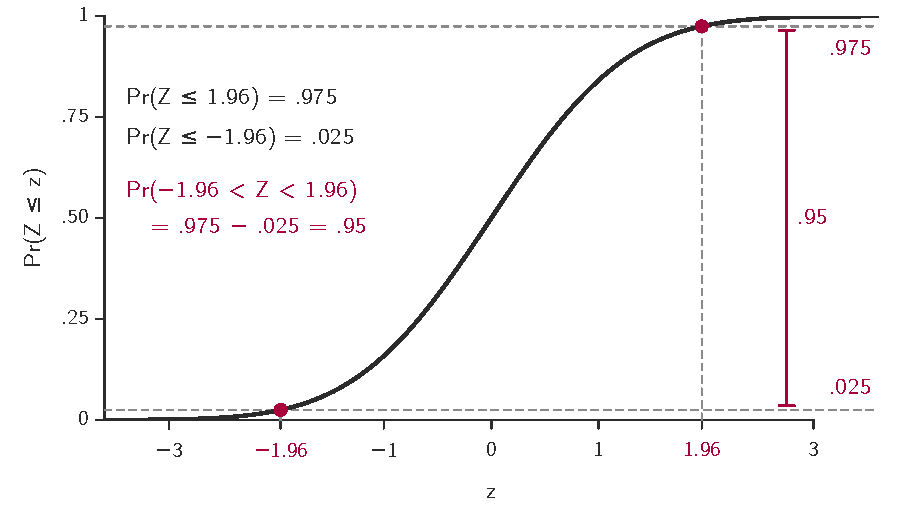
\includegraphics[height=0.82\textheight]{std_normal_cdf.pdf}
\end{figure}

}


\frame{
\frametitle{Constructing a Confidence Interval with Known $\sigma^2$}
So we know that:
$$\Pr\l(-1.96 < \frac{\overline{X}_n - \mu}{1/\sqrt{n}}  <1.96\r) \ = \ .95$$

Rearranging yields:
$$\Pr\l( \overline{X}_n -1.96/\sqrt{n} \ < \ \mu \ < \ \overline{X}_n + 1.96/ \sqrt{n}\r)
\ = \ .95
$$
\pause

This implies that the following interval estimator
$$
\l[\, \overline{X}_n -1.96/\sqrt{n}\, ,\, \overline{X}_n +1.96/\sqrt{n}\, \r]
$$
contains the true population mean $\mu$ with probability $0.95$. \\
\pause
\medskip

We call this estimator a 95\% \alert{confidence interval} for $\mu$.
}

\frame{
\frametitle{Interpreting a Confidence Interval}
\small
\begin{itemize}
\item Imagine we implement the interval estimator $\overline{X}_n \pm 1.96/\sqrt{n}$ for a particular sample and obtain the estimate of $[2.5, \ 3.3]$.
\item Does this mean that there is a .95 probability that the true parameter value $\mu$ lies between these two particular numbers? \pause No! \pause
  \item Confidence intervals are easy to construct, but difficult to interpret:
  \begin{itemize}
  \item Each confidence interval estima\underline{te} from a particular sample
  either contains $\mu$ or not \medskip
  \item However, if we were to repeatedly calculate the interval estima\underline{tor} over
  many random samples from the same population, 95\% of the time the constructed
  confidence intervals would cover $\mu$ \medskip
  \item Therefore, we refer to .95 as the \alert{coverage probability}
  \end{itemize}
\end{itemize}
}

\begin{frame}
\frametitle{Simulating Coverage Probability of Confidence Intervals}
100 samples of size 100 from $N(0, 1)$:
\vspace{-.4cm}
\begin{center}
\only<1|handout:0>{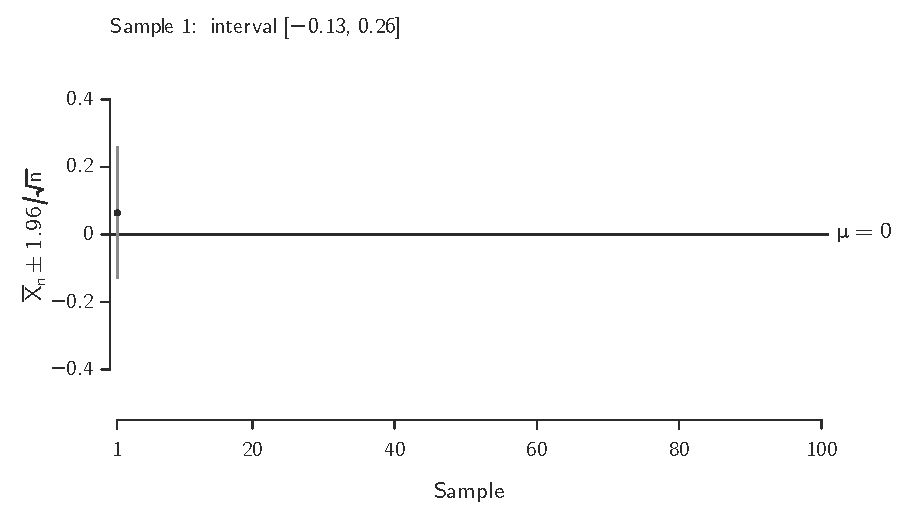
\includegraphics[height=0.80\textheight]{ci_sim_step1.pdf}}%
\only<2|handout:0>{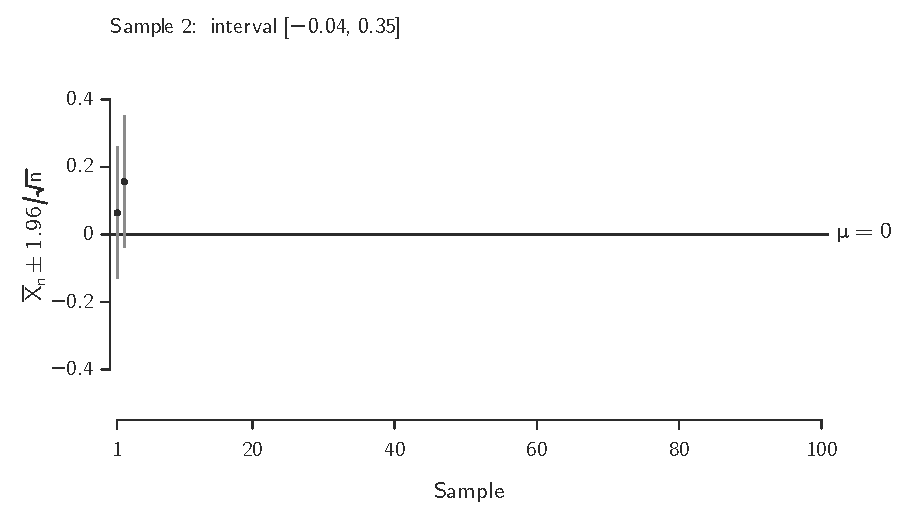
\includegraphics[height=0.80\textheight]{ci_sim_step2.pdf}}%
\only<3|handout:1>{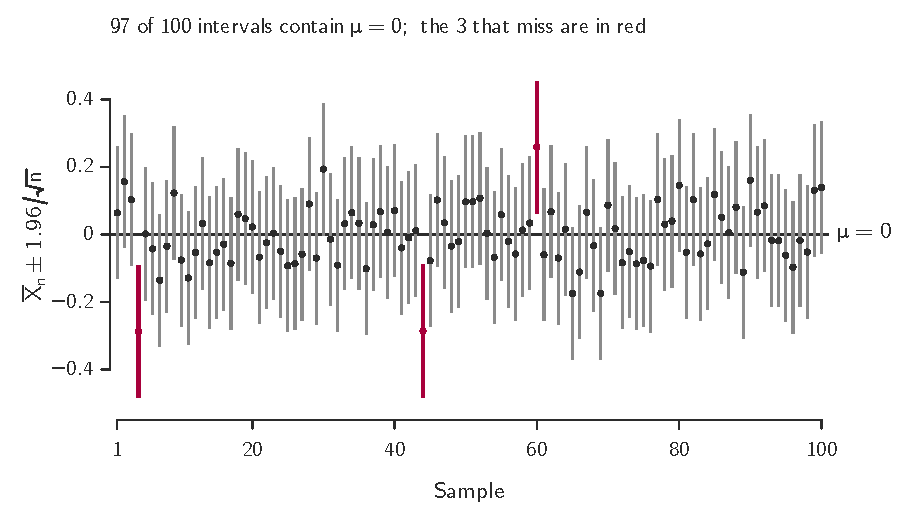
\includegraphics[height=0.80\textheight]{ci_sim_step3.pdf}}
\end{center}
\end{frame}

\frame{
\frametitle{Constructing a Confidence Interval with Known $\sigma^2$}

\begin{itemize}
  \item The same principle easily extends to normal populations with any known variance.
\medskip
  \item If $X \stackrel{iid}{\sim} N(\mu,\sigma^2)$ and we draw an i.i.d. random sample of size $n$,
  $X_1,...,X_n$, a 95\% confidence interval for the population mean $\mu$
  is:
$$
\l[\overline{X}_n -1.96 \sigma/\sqrt{n}, \ \overline{X}_n + 1.96 \sigma/ \sqrt{n}\r] $$
\pause
\vspace{-.5\baselineskip}
  \item More generally, a $100(1-\alpha)$\% confidence interval for $\mu$ is
$$
\l[\overline{X}_n - z_{\alpha/2}\, \sigma/\sqrt{n}, \ \overline{X}_n + z_{\alpha/2}\, \sigma/ \sqrt{n}\r]
$$
where $z_{\alpha/2}$ is the $100(1-\alpha/2)$ percentile of the standard normal distribution.
\end{itemize}
\vspace{-.5\baselineskip}
\begin{columns}
\column{.4\textwidth}
{\footnotesize
\begin{center}
\begin{tabular}{ccc}
 \hline
  \alert{Confidence level} & $\alpha$ & $z_{\alpha/2}$ \\
  \hline
  90\% & .1  & 1.645 \\
  95\% & .05 & 1.960 \\
  99\% & .01  & 2.576 \\
  \hline
\end{tabular}
\end{center}
}

\column{.4\textwidth}
\begin{center}
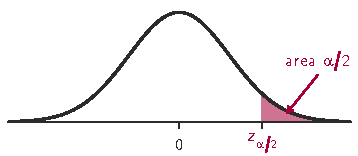
\includegraphics[width=\textwidth]{z_upper_tail}
\end{center}
\end{columns}

}



\begin{frame}[fragile]
\frametitle{Example: Feeling Thermometer Scores in ANES 2020}

\begin{footnotesize}
\begin{verbatim}
==============================================================
      INTRO PRE-ELECTION POLITICAL FIGURE THERMOMETERS
==============================================================

I'd like to get your feelings toward some of our political
leaders and other people who are in the news these days. I'll
read the name of a person and I'd like you to rate that
person using something we call the feeling thermometer.
Ratings between 50 degrees and 100 degrees mean
that you feel favorable and warm toward the person.
Ratings between 0 degrees and 50 degrees mean that you
don't feel favorable toward the person and that you
don't care too much for that person. You would
rate the person at the 50 degree mark if you don't feel
particularly warm or cold toward the person.

How would you rate:  Joe Biden       (V201151)
How would you rate:  Donald Trump    (V201152)
\end{verbatim}
\end{footnotesize}
\slidesource{American National Election Studies. 2021. ANES 2020 Time Series Study Full Release [dataset and documentation]. February 10, 2022 version. \href{https://electionstudies.org/data-center/2020-time-series-study/}{electionstudies.org/data-center/2020-time-series-study}}
\end{frame}

\frame{
\frametitle{Empirical Distribution of FT Scores}
\begin{center}
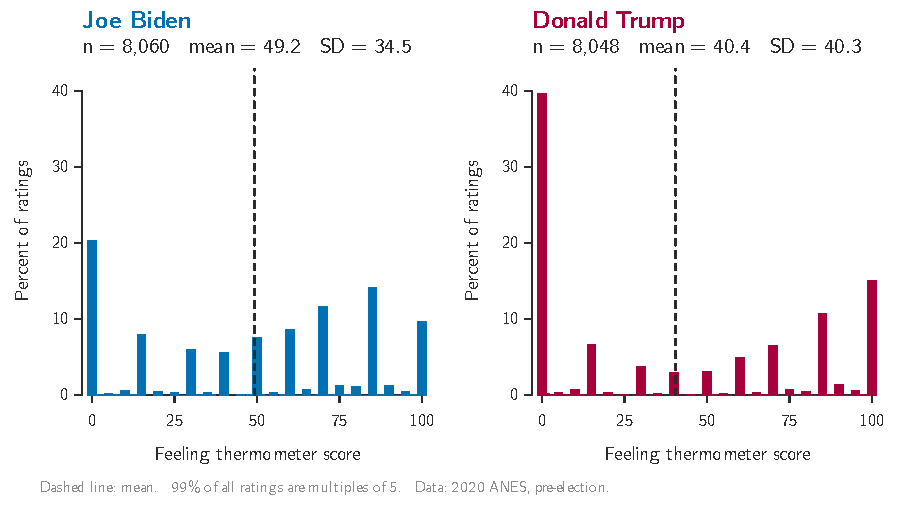
\includegraphics[height=0.82\textheight]{ft_distribution.pdf}
\end{center}
}

\frame{
\frametitle{Feeling Thermometer Example: Normal \&  Known Variance}
Assume (for now) that Biden's FT scores are (1) normally distributed and (2) we
(somehow) know that $\sigma = 34.5$. \\

\bigskip

We treat the ANES respondents as an i.i.d.\ sample, ignoring the survey weights and sampling design: $n=8{,}060$ respondents rated Biden, with sample mean FT score $\overline{X}_n=49.24$.
\\

\bigskip

Q. What is the 95\% confidence interval for the true mean FT score for Biden?\\

\bigskip \pause

A. Plug $n=8{,}060$, $\sigma = 34.5$ and $\overline{X}_n=49.24$ in:
$$\l[\overline{X}_n -1.96 \sigma/\sqrt{n}, \ \overline{X}_n + 1.96 \sigma/\sqrt{n}\r]$$ \pause
\vspace{-\baselineskip}
$$ = \ \l[49.24 -1.96 \cdot 34.5/\sqrt{8{,}060}, \ 49.24 +1.96 \cdot 34.5/\sqrt{8{,}060}\r] $$
$$ = \ \l[48.49, \ 49.99\r]$$

}

\frame{
\frametitle{Example: FT Scores Interval Estimates}
\begin{center}
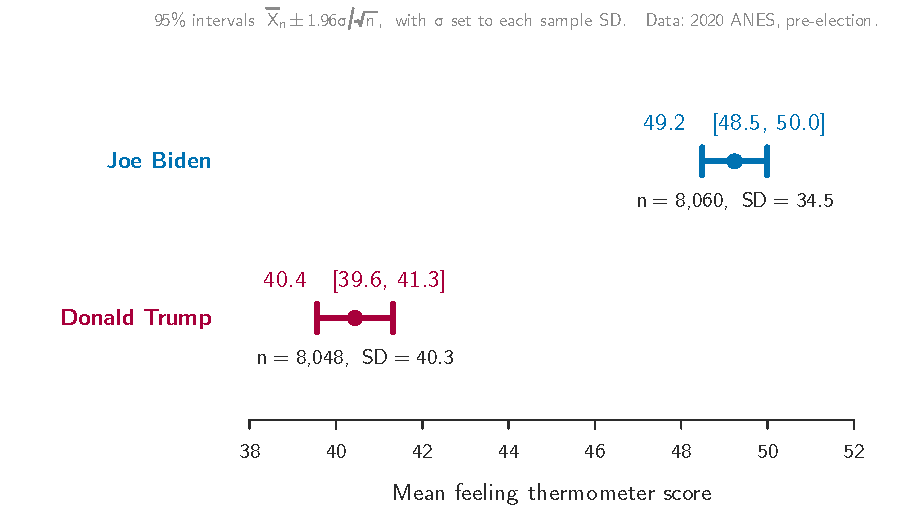
\includegraphics[height=0.82\textheight]{ft_intervals.pdf}
\end{center}
}


\section{Mean of Normal Population with Unknown Variance}

\frame{
\frametitle{Normal Population with Unknown $\sigma^2$}

In practice, it is rarely the case that we somehow know the true value of $\sigma^2$. \\
\pause \medskip

Suppose now that we have an i.i.d. random sample $X_1,...,X_n$ from
$X \stackrel{iid}{\sim} N(\mu,\sigma^2)$, where $\sigma^2$ is \alert{unknown}.
Then, as before,
$$
\overline{X}_n\sim N(\mu,\sigma^2/n) \quad \text{and so} \quad \frac{\overline{X}_n - \mu}{\sigma/\sqrt{n}} \sim N(0,1).
$$
\medskip \pause
Previously, we then constructed the interval:
$$
\l[\overline{X}_n - z_{\alpha/2} \sigma/\sqrt{n}, \ \overline{X}_n + z_{\alpha/2} \sigma/\sqrt{n}\r]
$$
But we can \textbf{not} directly use this now because \pause $\sigma^2$ is unknown. \\ \pause
\medskip
Instead, we need an \alert{estimator} of $\sigma^2$, $\hat\sigma^2$.

}





\frame{
\frametitle{Estimators for the Population Variance}
\small
Two possible estimators of population variance:
\begin{displaymath}
S_{0n}^2 = \frac{1}{n}\sum_{i=1}^n (X_i-\overline{X}_n)^2\qquad 
S_{1n}^2 = \frac{1}{n-1}\sum_{i=1}^n (X_i-\overline{X}_n)^2
\end{displaymath}
\medskip
Which do we prefer? \pause Let's check properties of these estimators. \textbf{Show (Worksheet Q1):} \pause
\begin{enumerate}
\item Unbiasedness: 
$$ E[S_{0n}^2] = \frac{n-1}{n}\sigma^2 \quad \text{and} \quad E[S_{1n}^2] = \sigma^2 $$
\pause
\vspace{-.5\baselineskip}
\item Consistency: 
$$ S_{0n}^2 \ \stackrel{p}{\to} \ \onslide<5>{\sigma^2} \quad \text{and} \quad S_{1n}^2 \ \stackrel{p}{\to} \ \onslide<5>{\sigma^2} $$
\end{enumerate} \pause
\vspace{-\baselineskip}
$S_{1n}^2$ (unbiased and consistent) is commonly called the \alert{sample variance}.
}


\frame{
\frametitle{Estimating $\sigma^2$ and the Standard Error}
We use the sample variance $S_n^2 \equiv S_{1n}^2$ to estimate the population variance $\sigma^2$.
(The plug-in (analogy-principle) estimator of the variance is $S_{0n}^2$; dividing by $n-1$ instead of $n$ corrects its bias.)
$$
S_n^2 = \frac{1}{n-1}\sum_{i=1}^n (X_i-\overline{X}_n)^2
$$
Our estimated standard deviation of the sampling distribution (i.e. estimated \alert{standard error}) of $\overline{X}_n$
is therefore $S_n/\sqrt{n}$.
\bigskip\pause

Does $\overline{X}_n \sim N(\mu, S_n^2/n)$, which would imply
$\frac{\overline{X}_n-\mu}{S_n/\sqrt{n}} \sim N(0,1)$? \\
\pause No, because $S_n$ is a random variable instead of a parameter (like $\sigma$).

\pause
\bigskip
Thus, we need to derive the sampling distribution of the new random variable
$$ T_n \ \equiv \ \frac{\overline{X}_n-\mu}{S_n/\sqrt{n}} \ \sim \ \text{\LARGE ?} $$
}


\frame{
\frametitle{Sampling Distribution with the Estimated Variance}
It turns out that $T_n$ follows \alert{Student's $t$-distribution} with $n-1$
\alert{degrees of freedom}, written $\tau_{n-1}$.
\begin{theorem}[Distribution of $t$-Value from a Normal Population]
Suppose we have an i.i.d. random sample of size $n$ from $N(\mu,\sigma^2)$.
Then, the sample mean $\overline{X}_n$ standardized with the estimated standard
error $S_n/\sqrt{n}$ satisfies,
$$ T_n \ \equiv \ \frac{\overline{X}_n-\mu}{S_n/\sqrt{n}} \ \sim \ \tau_{n-1} $$
\end{theorem}
\begin{itemize}
\item \textbf{Prove (Worksheet Q2)}
\item The quantity $T_n$ is commonly called the \alert{t-value}. It depends on the unknown $\mu$, but for a normal population its distribution does not depend on $\mu$ or $\sigma^2$.
\item Student's $t$-distribution has well known properties, and so can be used to
construct confidence intervals like $N(0,1)$.
\end{itemize}
}


\frame{
\frametitle{Properties of Student's $t$-Distribution}
\small
\vspace{-1.25\baselineskip}
\begin{center}
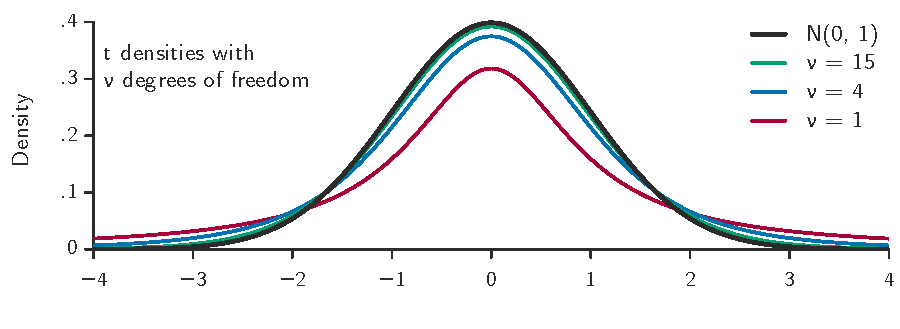
\includegraphics[height=.52\textheight]{t_densities.pdf}
\end{center}
\vspace{-1.5\baselineskip}
\begin{itemize}
  \item The shape of the $t$-distribution is determined by one parameter, $\nu$ (degrees of freedom)
  \item If $X \sim \tau_\nu$, then $E[X] = 0$ (for $\nu > 1$) and $V[X] = \nu/(\nu - 2)$ (for $\nu > 2$)
  \item Bell-shaped like the normal distribution, but has fatter tails for $\nu <\infty$
  \item $X \stackrel{d}{\rightarrow} N(0,1)$ as $\nu \to\infty$
  \item R functions: \texttt{dt(x, df)} (PDF), \quad \texttt{pt(q, df)} (CDF) \\
    \qquad \qquad \quad \texttt{qt(p, df)} (quantiles), \quad \texttt{rt(n, df)} (random draws)
\end{itemize}
}


\frame{
\frametitle{Constructing a Confidence Interval with Unknown $\sigma^2$}
\small
To calculate confidence intervals, we follow the same procedure as the case of
known variance, except that we now use percentiles of $t$ instead of $z$: $t_{\alpha/2,\nu}$ is the
$100(1-\alpha/2)$ percentile of $\tau_\nu$.
{\footnotesize
\begin{center}
\begin{tabular}{ccccccc}
 \hline
  \alert{Confidence level} & $\alpha$
                & $t_{\alpha/2,1}$ & $t_{\alpha/2,4}$ & $t_{\alpha/2,15}$ & $\cdots$ & $z_{\alpha/2}$ \\
  \hline
  90\% & .1  & 6.314 & 2.132 & 1.753 & $\cdots$ & 1.645 \\
  95\% & .05 & 12.71 & 2.776 & 2.131 & $\cdots$ & 1.960 \\
  99\% & .01 & 63.66 & 4.604 & 2.947 & $\cdots$ & 2.576 \\
  \hline
\end{tabular}
\end{center}
}
\pause
That is, we have
$$
\frac{\overline{X}_n - \mu}{S_n/\sqrt{n}} \ \sim  \ \tau_{n-1}
$$
So
$$\Pr\l(-t_{\alpha/2,(n-1)} < \frac{\overline{X}_n - \mu}{S_n/\sqrt{n}}  < t_{\alpha/2,(n-1)}\r) \ = \ 1-\alpha$$
$$\Longleftrightarrow \quad
 \Pr\l( \overline{X}_n - t_{\alpha/2,(n-1)}S_n/\sqrt{n} \ < \ \mu \ < \ \overline{X}_n + t_{\alpha/2,(n-1)}S_n/ \sqrt{n}\r)
\ = \ 1 - \alpha
$$

\medskip
\pause

Therefore, the $100(1-\alpha)$\% confidence interval for $\mu$ with unknown $\sigma^2$ is
$$
\l[ \overline{X}_n -t_{\alpha/2,(n-1)}S_n/\sqrt{n}, \ \overline{X}_n +t_{\alpha/2,(n-1)}S_n/\sqrt{n} \r]
$$

\pause
\medskip

A good rule of thumb for a 95\% C.I. for a typical sample size is $t_{\alpha/2,(n-1)} \approx 2$.

}

\frame{
  \frametitle{Worksheet Q3}

Suppose we have an i.i.d. random sample of size $n$, $X_1,...,X_n$, from $X \stackrel{iid}{\sim} N(\mu,\sigma^2)$. For constants $a,b$ with $b\neq0$, derive a $100(1-\alpha)\%$ confidence interval for $(a+b\mu)$ under 
\begin{itemize}
  \item[(i)] known $\sigma^2$
  \item[(ii)] unknown $\sigma^2$
\end{itemize}
}

\section{Mean of Population with Unknown Distribution}

\frame{
\frametitle{Asymptotic Confidence Intervals for Unknown Distribution}
\small
Often, observed distribution of $X$ is so far from normal that we do not want to assume
$X \sim N(\mu,\sigma^2)$ (e.g. Trump's FT scores). \\ \medskip

How can we proceed? \pause {\it The central limit theorem!} \pause \medskip

If $X_1,\dots,X_n$ are i.i.d. with finite variance $\sigma^2 > 0$, the CLT gives
$$ Z_n \ \equiv \ \frac{\overline{X}_n - \mu}{\sigma/\sqrt{n}} \quad \stackrel{d}{\longrightarrow} \quad N(0,1) $$
and we also know that
$$ S_n^2 \quad \stackrel{p}{\longrightarrow} \quad \pause \sigma^2 $$
as $n \to \infty$. \pause

\medskip

This therefore implies
$$ T_n \ \equiv \ \frac{\overline{X}_n - \mu}{S_n/\sqrt{n}} \quad \stackrel{d}{\longrightarrow} \pause \quad N(0,1) $$

\pause

{\bf Result:}\\
{\it If the sample is i.i.d. with finite variance, the normal interval
$\overline{X}_n \pm z_{\alpha/2}\, S_n/\sqrt{n}$ covers $\mu$ with probability close to $1-\alpha$
when $n$ is large, even if the population is not normal and $\sigma^2$ is unknown.}

}

\frame{
\frametitle{Using the $t$ Interval for Robust Inference}
The asymptotic normal confidence interval is convenient, but we must assume
that $n$ is large enough. \\ \medskip

If $n$ is small, the normal intervals are typically \alert{overconfident}, i.e. too narrow.
\\ \medskip \pause

To address this concern, some propose that we use the $t$ interval instead of normal. \\
\medskip

The logic:
\begin{itemize}
\item If $n$ is large, $t_{\alpha/2,(n-1)} \approx z_{\alpha/2}$ (1.984 vs.\ 1.960 at $n = 100$),
so the $t$ and normal intervals are nearly the same, and the CLT makes both valid.
\pause
\smallskip
\item If $n$ is small, the $t$ interval is wider than the normal interval, so it is less overconfident.
It can still cover $\mu$ less than 95\% of the time when the population is skewed (next slide).
\end{itemize}
\pause
Therefore, it is sensible to use the $t$ interval even if we do not assume that the
population distribution is normal, especially if $n$ is small.

}


\frame{
\frametitle{Simulation Study: 95\% Asymptotic Confidence Interval}
\small
Population: $X\sim Exp(\mu=1)$ (Exponential Distribution with Mean of 1) \\
\onslide<2>{Coverage of the asymptotic confidence intervals as $n$ varies from $2$ to $400$}
\vspace{-\baselineskip}
\begin{figure}[ht] \centering
        \only<1|handout:0>{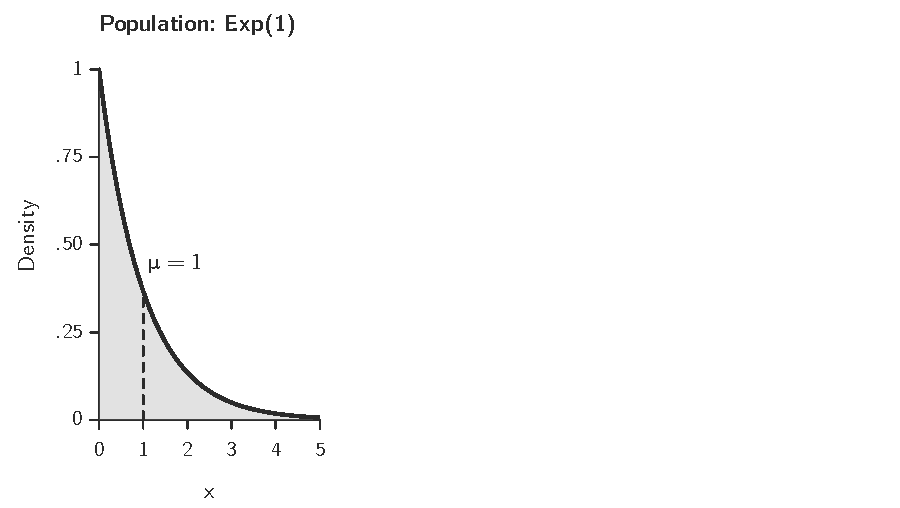
\includegraphics[height=0.74\textheight]{exp_coverage_step1.pdf}}%
        \only<2|handout:1>{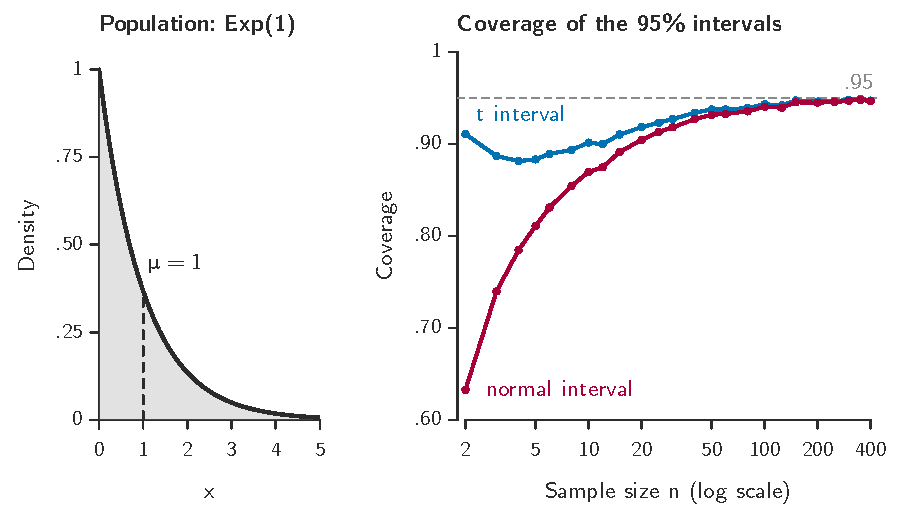
\includegraphics[height=0.74\textheight]{exp_coverage_step2.pdf}}
\end{figure}

}


\section{Summary}

\frame{
\frametitle{Summary:}
\small
To calculate a confidence interval for the population mean:
\medskip
\begin{itemize}
\item If we can safely assume that the population is normal (rather unlikely),
\medskip
    \begin{itemize}
    \addtolength{\itemsep}{.5\baselineskip}
    \item Use the \alert{normal interval} if the variance is also known (even less likely)
    \item Use the \alert{$t$ interval} if the variance has to be estimated from data.
    \end{itemize}
\pause
\bigskip
\item If we do not want to assume a normal population distribution,
\medskip
    \begin{itemize}
    \addtolength{\itemsep}{.5\baselineskip}
    \item Use either the \alert{normal interval} or \alert{$t$ interval} (choice doesn't matter) if sample size is large ($n > 100$ or so)
    \item Use the \alert{$t$ interval} if sample size is medium (about $20 \leq n \leq 100$)
    \item If sample size is smaller than that ($n < 20$) for now also use \alert{$t$ interval}---more on this later in methods sequence
    \end{itemize}
\end{itemize}
\medskip
Keep in mind that it is almost always better to be conservative when it comes to statistics.
}



\end{document}
